\documentclass[tikz]{standalone}
\usepackage{pgfplots}
\pgfplotsset{compat=1.15}
\usepackage{mathrsfs}
\usetikzlibrary{arrows,calc}
\usepackage{tkz-euclide}
\pagestyle{empty}
\usepackage{fp}

\definecolor{AngleClr}{rgb}{0,0.39215686274509803,0}
\definecolor{ShapeClr}{rgb}{0.6,0.2,0}

\begin{document}

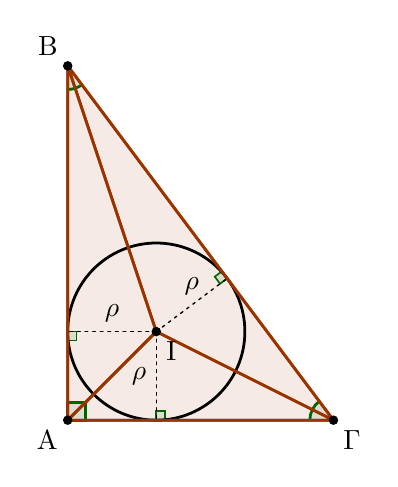
\begin{tikzpicture}[scale=.75]
\tkzSetUpLine[line width=1pt,color=black]
\tkzSetUpPoint[fill=black]

\def\Scale{1.5}
\FPeval{\By}{4 * \Scale}
\FPeval{\Cx}{3 * \Scale}
\FPeval{\D}{5 * \Scale}
\FPeval{\Rr}{(\By + \Cx - \D) / 2}

\tkzDefPoints{0/0/A,0/\By/B,\Cx/0/C,\Rr/\Rr/R,0/\Rr/Rx,\Rr/0/Ry}

\tkzDefPointBy[projection=onto B--C](R)\tkzGetPoint{H}

\tkzFillPolygon[fill=ShapeClr,fill opacity=0.1](A,B,C)
\tkzMarkRightAngle[line width=1pt, size=.3,color=AngleClr,fill=AngleClr,fill opacity=0.1](B,A,C)
\tkzFillAngles[fill=AngleClr,size=.4,fill opacity=0.1](A,B,C B,C,A)
\tkzMarkAngles[line width=1pt,size=.4,color=AngleClr](A,B,C B,C,A)

\tkzMarkRightAngles[line width=0.6pt, size=.15,color=AngleClr,fill=AngleClr,fill opacity=0.1](R,H,B A,Rx,R C,Ry,R)

\tkzDrawCircle[color=black,line width=1pt](R,Rx)
\tkzDrawSegments[line width=0.5pt,color=black,dashed,dash pattern=on 1pt off 1.75pt](R,Rx R,Ry R,H)

\tkzDrawPolygons[color=ShapeClr](A,B,C A,B,R A,C,R B,C,R)

\tkzDrawPoints[size=3](A,B,C,R)
\tkzLabelPoint[below left](A){$\rm A$}
\tkzLabelPoint[above left](B){$\rm B$}
\tkzLabelPoint[below right](C){$\rm \Gamma$};
\tkzLabelPoint[below right](R){$\rm I$}
\tkzLabelSegment[above](R,Rx){$\rho$}
\tkzLabelSegment[left](R,Ry){$\rho$}
\tkzLabelSegment[above](R,H){$\rho$}

\end{tikzpicture}

\end{document}
